
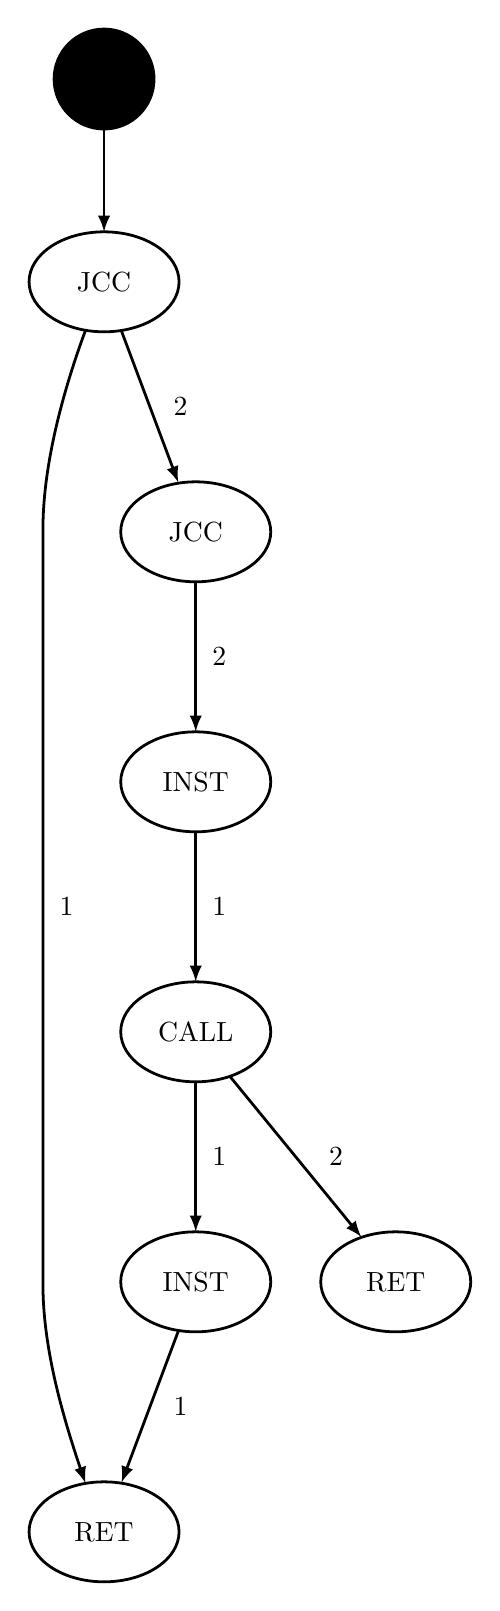
\begin{tikzpicture}[>=latex,line join=bevel,]
  \pgfsetlinewidth{1bp}
%%
\pgfsetcolor{black}
  % Edge: 2 -> 3
  \draw [->] (60bp,179.61bp) .. controls (60bp,167.24bp) and (60bp,150.37bp)  .. (60bp,126.05bp);
  \definecolor{strokecol}{rgb}{0.0,0.0,0.0};
  \pgfsetstrokecolor{strokecol}
  \draw (68.5bp,153bp) node {1};
  % Edge: 6 -> 7
  \draw [->] (60bp,359.61bp) .. controls (60bp,347.24bp) and (60bp,330.37bp)  .. (60bp,306.05bp);
  \draw (68.5bp,333bp) node {2};
  % Edge: 1 -> 6
  \draw [->] (33.207bp,450.45bp) .. controls (37.97bp,437.75bp) and (44.639bp,419.96bp)  .. (53.709bp,395.78bp);
  \draw (54.5bp,423bp) node {2};
  % Edge: 7 -> 2
  \draw [->] (60bp,269.61bp) .. controls (60bp,257.24bp) and (60bp,240.37bp)  .. (60bp,216.05bp);
  \draw (68.5bp,243bp) node {1};
  % Edge: 1 -> 4
  \draw [->] (20.28bp,450.44bp) .. controls (13.81bp,432.97bp) and (5bp,404.51bp)  .. (5bp,379bp) .. controls (5bp,379bp) and (5bp,379bp)  .. (5bp,107bp) .. controls (5bp,85.873bp) and (11.042bp,62.722bp)  .. (20.28bp,35.562bp);
  \draw (13.5bp,243bp) node {1};
  % Edge: 0 -> 1
  \draw [->] (27bp,522.81bp) .. controls (27bp,514.79bp) and (27bp,505.05bp)  .. (27bp,486.03bp);
  % Edge: 2 -> 5
  \draw [->] (72.541bp,181.67bp) .. controls (83.692bp,168.04bp) and (100.16bp,147.92bp)  .. (119.6bp,124.15bp);
  \draw (110.5bp,153bp) node {2};
  % Edge: 3 -> 4
  \draw [->] (53.793bp,90.448bp) .. controls (49.03bp,77.746bp) and (42.361bp,59.962bp)  .. (33.291bp,35.777bp);
  \draw (54.5bp,63bp) node {1};
  % Node: 1
\begin{scope}
  \definecolor{strokecol}{rgb}{0.0,0.0,0.0};
  \pgfsetstrokecolor{strokecol}
  \draw (27bp,468bp) ellipse (27bp and 18bp);
  \draw (27bp,468bp) node {JCC};
\end{scope}
  % Node: 0
\begin{scope}
  \definecolor{strokecol}{rgb}{0.0,0.0,0.0};
  \pgfsetstrokecolor{strokecol}
  \definecolor{fillcol}{rgb}{0.0,0.0,0.0};
  \pgfsetfillcolor{fillcol}
  \filldraw [opacity=1] (27bp,541bp) ellipse (18bp and 18bp);
\end{scope}
  % Node: 3
\begin{scope}
  \definecolor{strokecol}{rgb}{0.0,0.0,0.0};
  \pgfsetstrokecolor{strokecol}
  \draw (60bp,108bp) ellipse (27bp and 18bp);
  \draw (60bp,108bp) node {INST};
\end{scope}
  % Node: 2
\begin{scope}
  \definecolor{strokecol}{rgb}{0.0,0.0,0.0};
  \pgfsetstrokecolor{strokecol}
  \draw (60bp,198bp) ellipse (27bp and 18bp);
  \draw (60bp,198bp) node {CALL};
\end{scope}
  % Node: 5
\begin{scope}
  \definecolor{strokecol}{rgb}{0.0,0.0,0.0};
  \pgfsetstrokecolor{strokecol}
  \draw (132bp,108bp) ellipse (27bp and 18bp);
  \draw (132bp,108bp) node {RET};
\end{scope}
  % Node: 4
\begin{scope}
  \definecolor{strokecol}{rgb}{0.0,0.0,0.0};
  \pgfsetstrokecolor{strokecol}
  \draw (27bp,18bp) ellipse (27bp and 18bp);
  \draw (27bp,18bp) node {RET};
\end{scope}
  % Node: 7
\begin{scope}
  \definecolor{strokecol}{rgb}{0.0,0.0,0.0};
  \pgfsetstrokecolor{strokecol}
  \draw (60bp,288bp) ellipse (27bp and 18bp);
  \draw (60bp,288bp) node {INST};
\end{scope}
  % Node: 6
\begin{scope}
  \definecolor{strokecol}{rgb}{0.0,0.0,0.0};
  \pgfsetstrokecolor{strokecol}
  \draw (60bp,378bp) ellipse (27bp and 18bp);
  \draw (60bp,378bp) node {JCC};
\end{scope}
%
\end{tikzpicture}

